\section{Présentation du port}

\begin{frame}{Le terminal à conteneurs sud}
  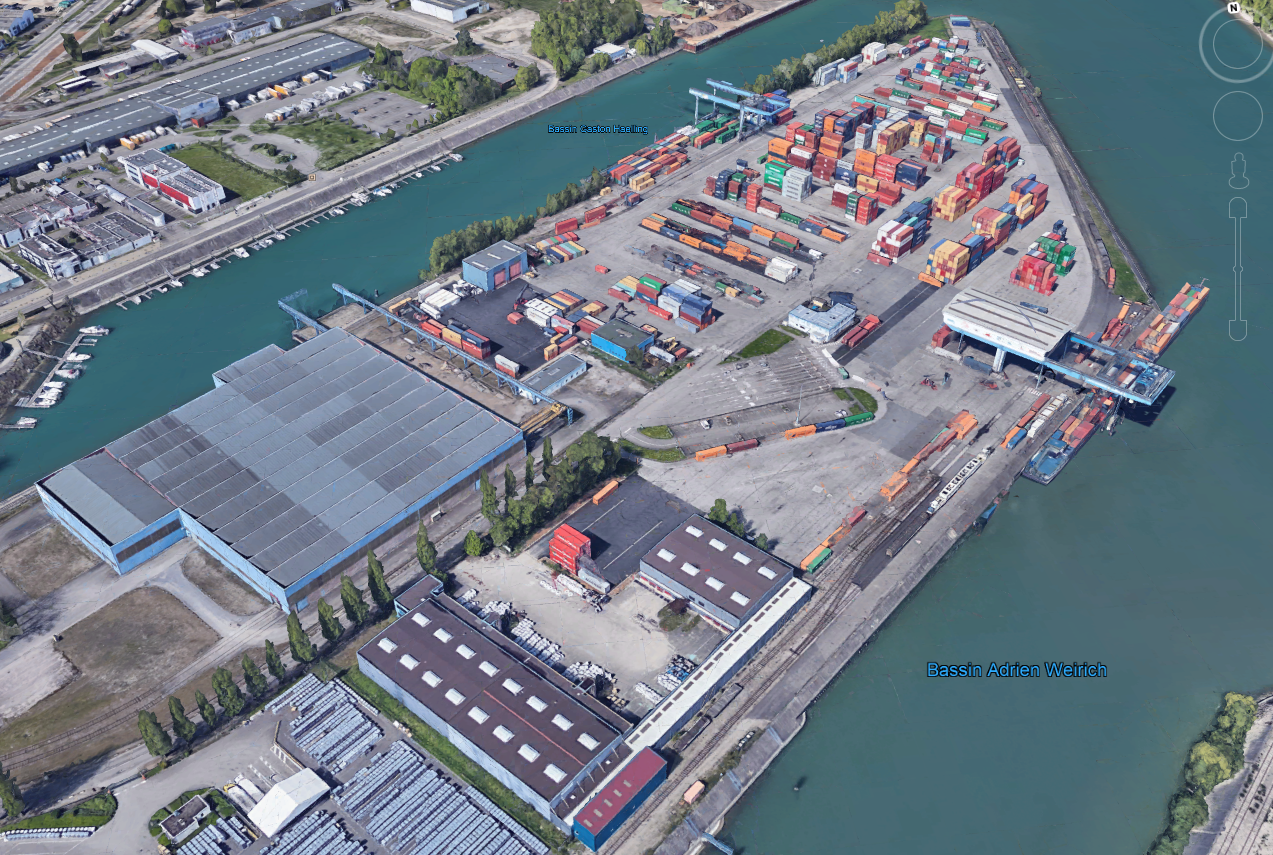
\includegraphics[width=\textwidth]{../images/image14}
\end{frame}

\begin{frame}{Le terminal à conteneurs sud}
  \begin{itemize}
  \item Infrastructures et outillage
    \begin{itemize}
    \item
      2 portiques fluviaux à conteneurs, mobiles
    \item
      1 portique fluvial à colis lourds (capacité 460 tonnes)
    \item
      1 420 mètres de linéaire ferroviaire en 4 voies de longueur variant entre 330 et 400 mètres
    \item
      8 reach-stackers
    \item
      itinéraires routiers adaptés aux colis lourds
    \item
      systèmes informatiques intégrés (TOS)
    \item
      superficie : 10 ha
    \end{itemize}
  \item Enjeux
    \begin{itemize}
    \item Congestion de poids lourds
    \item Elargissement sur un terrain adjacent pour améliorer la fluidité des trafics
    \end{itemize}
  \end{itemize}
\end{frame}

\begin{frame}{Problèmatique du PAS}
      \begin{itemize}
      \item Trafic 2016-2017: 128 500 conteneurs (en UTI)
      \item donnt 91000 vides avec la politique du First In, First Out
      \item aucune visibilité sur la date de sortie des conteneurs
      \item coût d'un stacker:
        \begin{itemize}
        \item 400 000\euro{}  HT à l'achat
        \item 1 pneu = 4 000\euro{} / unite (par 6)
        \item coût horaire: 60\euro{}  environ
        \end{itemize}
      \end{itemize}
      
      Le cout des stackers revient à 600 000\euro{}  par an.\\
      Un gain de 15\% en distance parcouru par les stackers représente une économie de 100 000\euro.
\end{frame}

\begin{frame}{Problèmatique du PAS}
  \begin{columns}
    \begin{column}{0.7\textwidth}
      Les conteneurs sont stockés par bloc, de manière à respecter la régle du FIFO.\\
      La gestion des blocs est gérée par leur système informatique (TOS).\\
      On peut donc ne pas considérer la hauteur des piles et se ramener à un problème 2D.
    \end{column}
    \begin{column}{0.3\textwidth}
      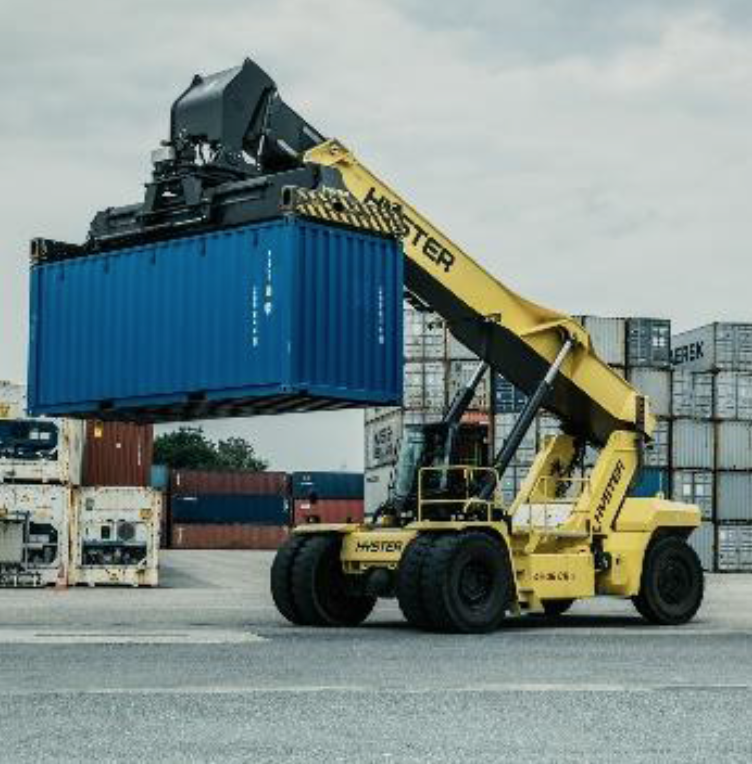
\includegraphics[width=\textwidth]{../images/PAS_stacker}
    \end{column}
  \end{columns}
  \vfill
  Le problème revient donc à répartir les travées de manière optimale sur la surface du port.\\
  Besoin d'avoir des travées de largeur suffisante pour maximiser l'espace utilisé, mais aussi de garder des travées pour les petits clients.
\end{frame}
